% ===================== 担当C =====================
\section{担当C — 楽譜・演奏制御}

\subsection{部品一覧}
担当Cで必要となる器具と環境について表\ref{need}に記す．

\begin{table}[H]
  \centering
  \caption{事前に揃えるべき器具・環境}
  \label{need}
  \begin{tabular}{|c|c|c|}
\hline
品目 & 数量 & 用途 \\\hline \hline
Arduino Uno R4 Wifi（子機用） & 5 & 楽器ユニット各1台 \\ \hline
USB Type-Cケーブル & 5 & 各子機とPC缶のSerial通信 \\ \hline
シリアル通信テスト環境（Arduino IDE シリアルモニタ）& - & C1テスト（B-C間遅延測定） \\ \hline
  \end{tabular}  
\end{table}



%\subsection{ハードウェア設計}
%（ここに記載）

\subsection{ソフトウェア設計}
%\subsubsection{ファイル構成}
%（ここに記載）

\subsubsection{楽譜データ構造}
本システムで実装する楽譜データ構造は音名インデックス，音の強さ，拍数の3要素を持つ二次元配列として定義する．音名インデックスの定義一覧は以下の通りである．\\

音名インデックス：$C4=0，D4=1，E4=2，F4=3，G4=4，A4=5（休符：6）$\\

定義例はソースコード\ref{index}の通りである．各パートの最後は休符を設定する．

\begin{figure}[H]
\renewcommand{\lstlistingname}{ソースコード}
    \begin{lstlisting}[
        language=C++,
        caption={楽譜配列（カエルの歌）},
        label=index,
        escapechar=@,
        frame=single,
        basicstyle=\ttfamily\small,
        breaklines=true
    ]
const uint8_t score[][3] = {
   {0, 100, 1},   //ド
   {1, 100, 1},   //レ
   {2, 100, 1},   //ミ
   {3, 100, 1},   //ファ
   // ... 以下省略（前章節分を定義）
   };
   
   const int SCORE_LEN = sizeof ( score ) / sizeof ( score [0] ) ;

   \end{lstlisting}
\end{figure}

\subsubsection{テンポ管理・演奏制御用の定数}
各楽器の演奏開始は親機からの輝度キューによって決定される．子機は自機IDに対応する輝度レベルを検出した時点でスタートフラグを立て，次の拍タイミングで演奏を開始する．演奏予定順序を参考として表\ref{offset02}に示す．
\begin{table}[H]
  \centering
  \caption{演奏予定順序（親機から動的に指示）}
  \label{offset02}
  \begin{tabular}{|c|c|c|}
\hline
楽器 & 演奏開始 & パート \\\hline \hline
ハイハット・シンバル & 0小節目 & リズム１ \\ \hline
バス・スネア & 0小節目 & リズム２ \\ \hline
鉄琴 & 2小節目 & 主旋律１ \\ \hline
ピアノ & 4小節目 & 主旋律２ \\ \hline
トランペット & 6小節目 & 主旋律３ \\ \hline
  \end{tabular}  
\end{table}
\FloatBarrier

小節管理に使用する定数はソースコード\ref{beat}の通りである．
\begin{figure}[H]
\renewcommand{\lstlistingname}{ソースコード}
    \begin{lstlisting}[
        language=C++,
        caption={小節管理の定数},
        label=beat,
        escapechar=@,
        frame=single,
        basicstyle=\ttfamily\small,
        breaklines=true
    ]
    
    const uint8_t BEATS_PER_BAR = 4;  //小節あたりの拍数
    
   \end{lstlisting}
\end{figure}

演奏テンポ一覧は表\ref{temp}の通りである．

\begin{table}[h]
  \centering
  \caption{演奏テンポ一覧表}
  \label{temp}
  \begin{tabular}{|c|c|}
\hline
区間 & テンポ  \\\hline \hline
開始〜14小節（一周目演奏終了） & 80bpm \\ \hline
15小節目（二周目演奏開始）以降 & 104bpm  \\ \hline

  \end{tabular}  
\end{table}
\FloatBarrier

テンポ管理は小節カウンタ（ソースコード\ref{beat}）による自立管理を行う．定義例はソースコード\ref{テンポ切替}の通りである．
\begin{figure}[H]
\renewcommand{\lstlistingname}{ソースコード}
    \begin{lstlisting}[
        language=C++,
        caption={テンポ切替定数},
        label=テンポ切替,
        escapechar=@,
        frame=single,
        basicstyle=\ttfamily\small,
        breaklines=true
    ]
    
    const uint16_t TEMPO_SLOW = 750;  //80bpm->拍間隔750ms
    
    const uint16_t TEMPO_FAST = 577;  //104bpm->拍間隔577ms
    
    const uint8_t TEMPO_CHANGE_BAR = 15;  //15小節目からTEMPO_FASTへ切替
    
    uint16_t currentInterval = TEMPO_SLOW;  //現在の拍間隔[ms]
    uint8_t barCount = 0;  //現在の小説カウンタ
    
   \end{lstlisting}
\end{figure}




\subsubsection{オブジェクト設計（クラス図）}

プログラム内で扱う変数一覧について表\ref{variable}に記す．
\begin{table}[H]
  \centering
  \caption{変数一覧}
  \label{variable}
  \begin{tabular}{|c|c|c|}
\hline
型 & 変数名 & 用途 \\\hline \hline
int & noteIndex = 0 & 現在の音符ポインタ \\ \hline
int & beatCount = 0 & 経過拍数 \\ \hline
int & remainBeats = 0 & 現在の音符の残り拍数 \\ \hline
bool & playing = false & 演奏フラグ（輝度キュー受信後に"true"になる） \\ \hline
bool & fermata = false & フェルマータ中フラグ \\ \hline
  \end{tabular}  
\end{table}







\subsubsection{関数設計}

本システムで実装する関数シグネチャと引数，戻り値，処理内容の一覧について表\ref{functions}に記す．特に複雑な関数（onBeatDetected()，advanceNote()）のフローチャートをそれぞれ図\ref{onBeatDetected}，\ref{advanceNote}に示す．


% プリアンブルに \usepackage{tabularx} が必要
\begin{table}[H]
  \centering
  \caption{関数一覧}
  \label{functions}
  \begin{tabularx}{\textwidth}{|p{4cm}|X|p{2cm}|X|}
    \hline
    関数名 & 引数 & 戻り値 & 処理内容 \\ \hline \hline
 %   bool detectBeat() & なし（void）&bool（ true / false )& フォトトランジスタで親機LEDを検出しtrueを返す．そうでない場合はfalseを返す． \\ \hline
    void onBeatDetected() & なし（void）& なし（void）& 拍検出時の処理：輝度キュー受信によるスタートフラグ確認，テンポ切替，音符更新・送信，前の音の停止の送信を実行 \\ \hline
    void advanceNote() & なし（void）& なし（void）& 残り拍数を減らし，0になったらnoteIndexを進める \\ \hline
    void sendCurrentNote() & なし（void）& なし（void）& score[noteIndex] からNOTE ON パケットを生成し送信する \\ \hline
    void sendNoteOn(uint8\_t note, uint8\_t vel) &uint8\_ note：音名インデックス（0~127　休符=255）　uint8\_vel：音の強さ（0~127）& なし（void）& 演奏用ArduinoからProcessingへシリアル送信する \\ \hline
    void onFermata() & なし（void）& なし（void）& フェルマータ受信時，次の拍を検出するまでプログラムを停止する \\ \hline
    void checkTempoChange() & なし（void）& なし（void）& barCountに応じてcurrentIntervalを切り替える \\ \hline
  \end{tabularx}  
\end{table}


\begin{figure}[H]
    \centering
    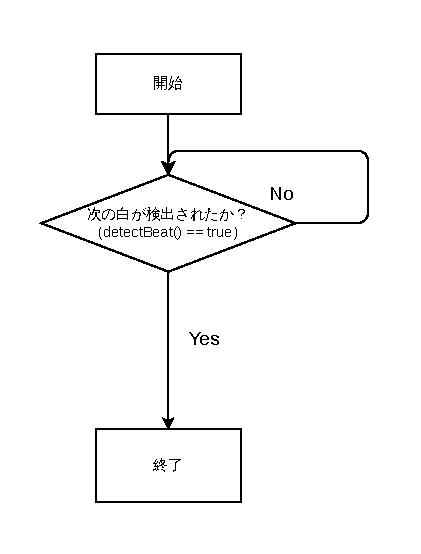
\includegraphics[width=0.8\linewidth, keepaspectratio]{figures/tantoC/onBeatDetected_drawio.pdf}
    \caption{フローチャート：onBeatDetected()}
    \label{onBeatDetected}
\end{figure}


\begin{figure}[H]
    \centering
    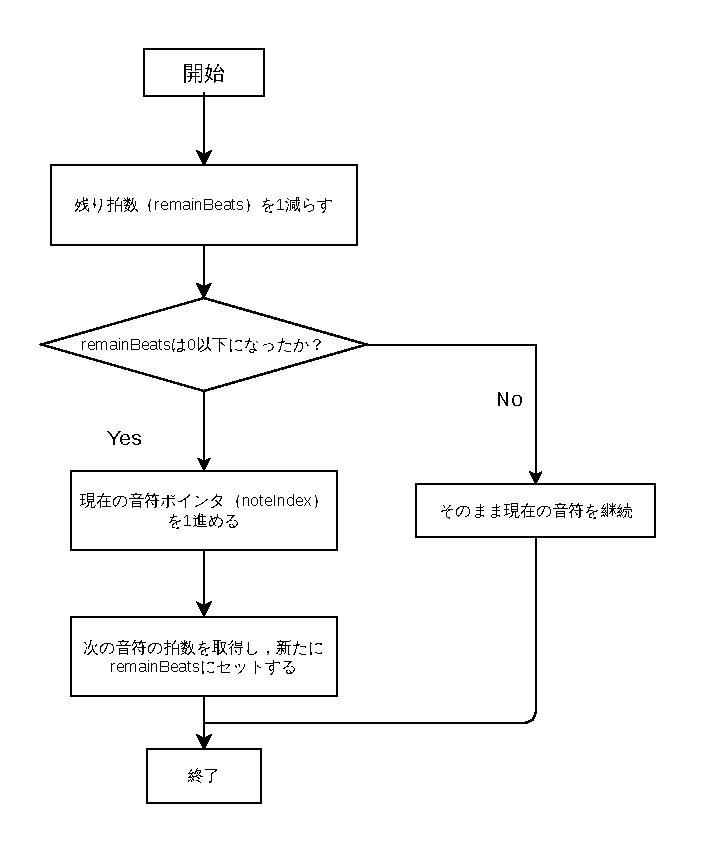
\includegraphics[width=0.6\linewidth, keepaspectratio]{figures/tantoC/advanceNote_drawio.pdf}
    \caption{フローチャート：advanceNote()}
    \label{advanceNote}
\end{figure}




\FloatBarrier



%\subsection{処理フローの設計}

%\figspace[4]{処理フロー図を挿入}

\subsection{テストの設計}
本システムの課題として，シリアル通信時の遅延と音声出力時の遅延が考えられる．そのため，結合テストとしてArduino-Processing 間の往復遅延測定を行い，遅延補正値の測定・定数化を行う．

